\ifdefined\XeTeXrevision\else\pdfoutput=1\fi
\documentclass[11pt]{article}
\usepackage[margin=1in]{geometry}
\usepackage{booktabs}
\usepackage{amsmath}
\usepackage{graphicx}
\usepackage{xcolor}
\usepackage{hyperref}
\usepackage{microtype}
\hypersetup{colorlinks=true, linkcolor=blue!60!black, citecolor=blue!60!black,
  urlcolor=blue!60!black, pdftitle={The Third Block Composes},
  pdfauthor={Franci Penov}}
\title{The Third Block Composes:\\One-Writer Bridges for Multi-Sensor Conditioning\\of a Frozen Language Model}
\author{Franci Penov \\ kortexa.ai \\ \texttt{francip@kortexa.ai}}
\date{2026-08-09}

\begin{document}
\maketitle

\begin{abstract}
Papers 7--9 closed every merged-writer route to composing sensor bricks on
a frozen language model: additive weight-space merges, shared-budget
activation merges, and cross-channel superposition all die by behavioral
dominance, and paper 10 located the deeper constraint --- the mode
structure of the joint utterance. This note reports the constructive
result those negatives were pointing at. Two structures no prior negative
tested --- \emph{one writer reading many sensors}, and
\emph{presence$\times$presence} joint behavior --- turn out to be
sufficient: a single hypernetwork bridge that reads two sensors' features
and emits one LoRA delta passes a registered gate at every (pair, seed)
cell at 4B (free-run joint-heed 0.75--1.00 against measured floors of
0.000--0.167), extends to \emph{three} sensors at 0.90 joint-heed in
every cell of both registered triples --- lifting the program's
longest-standing blocker, the third-block rail --- and promotes to a 27B
host with seven of nine cells passing outright (the creature pair perfect
at 1.000) and the two exceptions traced, row by row, to a state collision
in the shuffled control rather than to the bridge. Per-lane function is
retained everywhere, modality-dropout subsets behave as their subsets, and
the teacher-forced fit carries into free decode in every cell --- the
exact opposite of the self-bridge ladder's fate on the same host. The
practical claim: multi-sensor conditioning of a frozen model is solved at
the venues tested by giving the sensors one mouth-piece instead of asking
several to share a stage.
\end{abstract}

\section{The negatives that shaped the design}

The program has one composition result that always works --- selection
(paper 8) --- and a graveyard of superposition attempts. Paper 7: summed
weight-space deltas are provably lossless in the merge algebra and
behaviorally useless. Paper 9: two activation packets destroy each other
under a shared write budget, and block+packet pairs resolve by dominance,
dosed but not fungible. Paper 10: at 4B, even a single model cannot be
made to \emph{initiate} an utterance carrying recall and presence at
once. Every one of those failures shares two structural features: the
writers were trained independently and merged after the fact, and the
joint behavior asked for spanned two \emph{modes}. The design here
removes both: one bridge is trained \emph{natively} on the joint
behavior (no post-hoc merger exists to fight), and both contents are
present-tense states of the world (one mode, two facts).

\section{The harness}

Venues: frozen Qwen3.5-4B (March r4 blocks, the dispatch lanes' banks and
scorers) and frozen Qwen3.6-27B (the August r2 column). Registered pairs:
\texttt{temporal$+$vitals} (the creature's pair), \texttt{temporal$+$geo}
(both sinusoidal), \texttt{vitals$+$imu} (mixed encoder families).
Joint-heed means both lanes' registered scorers accept one free-decoded
utterance on held-out state pairs, under a neutral situation-naming
surface. M0 measured the floors decode-only before anything trained:
per-block solo, the paper-7 additive merge re-anchored in-band, a
prompt-only joint ask, and an oracle router (paper 8's ceiling, which
surfaces one lane by construction). \textbf{Every M0 cell at 27B is
0.000; at 4B everything is 0.000 except one flicker} (the
\texttt{vitals$+$imu} merge at 0.167, which does not
reproduce at 27B).

The joint bridge is deliberately boring: the house hypernetwork
(\texttt{BridgeHyper}) with a widened input --- two lanes' 256-d
features plus two presence bits --- emitting the same flat LoRA delta a
single block emits, trained by teacher-forced transcription of
machine-validated composed targets (both halves present-tense, four
validation rules, each rule tested to bite) with modality dropout 0.25 so
one artifact covers both subsets and the joint. Training runs through the
same autograd-safe injection path the evaluation uses. Gate per (pair,
seed): free-run joint-heed strictly above every M0 cell, per-lane
retention $\geq$ 0.80 of in-band solo, masked inputs reproduce solo
behavior, shuffled features at floor, zero-dose bit-exact identity,
byte-identical base weights.

\begin{figure}[t]
\centering
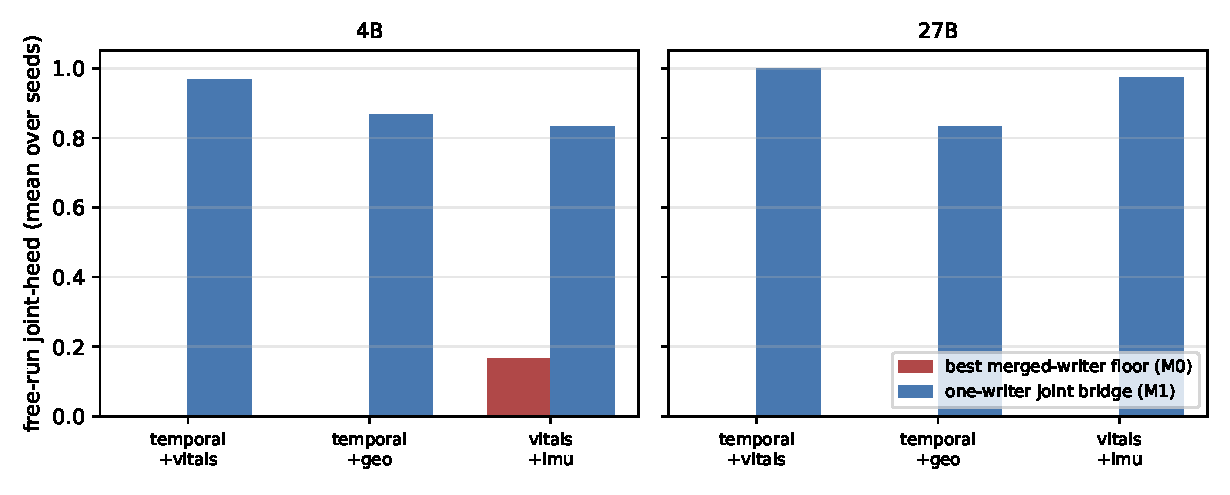
\includegraphics[width=\linewidth]{one-writer.pdf}
\caption{The one-writer result against the merged-writer floors, both
venues. Bars: best M0 floor per pair (max over solo, additive merge,
prompt-joint, router-oracle) vs the M1 joint bridge's free-run joint-heed
(mean over three seeds, $\beta$=1).}
\label{fig:onewriter}
\end{figure}

\section{Results}

\textbf{M1 at 4B: nine of nine cells pass.}
Table~\ref{tab:m1} column three carries the headline; the fit column
carries the contrast with paper 10 --- token accuracy 0.94--0.98
\emph{and the behavior transfers to free decode}, no cell showing the
teacher-forced/free-run gap that killed the self-bridge ladder on this
same host.

\begin{table}[t]
\centering
\small
\setlength{\tabcolsep}{4pt}
\begin{tabular}{lrrrrrr}
\toprule
pair & M0 floor & joint by seed & A heed & B heed & fit & passed \\
\midrule
\texttt{temporal$+$vitals} & 0.000 & 0.90/1.00/1.00 & 1.00--1.00 & 0.90--1.00 & 0.94--0.96 & 3/3 \\
\texttt{temporal$+$geo} & 0.000 & 0.90/0.80/0.90 & 1.00--1.00 & 0.80--0.90 & 0.97--0.98 & 3/3 \\
\texttt{vitals$+$imu} & 0.167 & 0.92/0.75/0.83 & 0.83--1.00 & 0.83--1.00 & 0.95--0.97 & 3/3 \\
\bottomrule
\end{tabular}
\caption{M1 at 4B, free-run joint-heed at $\beta$=1 per seed.}
\label{tab:m1}
\end{table}

\textbf{M1b: the third block composes.} The same mechanics at $N$=3
(three features, three presence bits, seven dropout subsets): joint-heed
--- all three lanes' scorers on one utterance --- is
\textbf{0.90 in every cell of both triples}, the
creature's tuple \texttt{temporal$+$vitals$+$geo} and the mixed-family
\texttt{temporal$+$vitals$+$imu}, against in-band triple additive-merge
floors of 0.000 (Table~\ref{tab:m1b}). The third-block rail --- the
named blocker behind the continuous self-loop, the personality block, and
multi-brick serving --- lifts at 4B under one writer.

\begin{table}[t]
\centering
\small
\begin{tabular}{lrrrr}
\toprule
triple & pairwise floor & triple merge & joint by seed & passed \\
\midrule
\texttt{temporal$+$vitals$+$geo} & 0.000 & 0.000 & 0.90/0.90/0.90 & 3/3 \\
\texttt{temporal$+$vitals$+$imu} & 0.167 & 0.000 & 0.90/0.90/0.90 & 3/3 \\
\bottomrule
\end{tabular}
\caption{M1b at 4B: three sensors, one writer.}
\label{tab:m1b}
\end{table}

\textbf{Promotion to 27B: seven of nine outright, and a control lesson.}
\texttt{temporal$+$vitals} is perfect (1.000 at every seed);
\texttt{vitals$+$imu} passes everywhere
(0.92/1.00/1.00);
\texttt{temporal$+$geo} runs
0.80/0.80/0.90 joint with full retention but
2 of its seeds recorded as non-passes on one check:
\texttt{shuffled\_at\_floor}. The row-level diagnosis is exact. The
shuffle rotated items by one; six of ten held-out pairs share the
temporal state under round-robin pairing, and the only joint hits --- the
same single item at both failing seeds, identical response text --- sit
on those collisions, against a floor of exactly 0.0. A 27B expresses a
partially-right packet where a 4B cannot. The cells stand as recorded
(the gate is the gate); the harness's shuffle is now a state-derangement,
and the claim rests on the seven clean cells.

\section{What this does and does not establish}

It establishes that the merged-writer negatives were about the
\emph{merge}, not about multi-sensor conditioning: give N sensors one
trained mouth-piece and a frozen host says both --- or all three ---
things at once, message-dependently, with each lane's function intact,
at 4B and at 27B. It also quietly confirms paper 10's mode account from
the constructive side: presence$\times$presence composes on the exact
host where recall$\times$presence would not compose under any
manipulation tested. It does \emph{not} yet attribute the win between
``one writer'' and ``natively-trained joint data'' --- the registered
depth-partition control (M3: independently-trained blocks on disjoint
layers, merged) runs next and is designed to separate exactly that pair
of explanations; the modality-dropout subsets already show the single
writer behaving as each solo when asked to. And $N$ beyond three, other
lane families, and serving integration remain open.

\section{Reproducibility}

Artifacts \texttt{multi-sensor-m0-\{4b,27b\}},
\texttt{multi-sensor-m1-\{4b,27b\}} and \texttt{multi-sensor-m1b-4b}
are bundled beside this note; every number and the figure render from
them alone. Harness: \texttt{tracks/multi-sensor/multi\_sensor.py};
registrations, results, and the two pre-run amendments in the track's
\texttt{PLAN.md}, each dated before its run.

\begin{thebibliography}{9}
\bibitem{penov2026interference} F.~Penov. Zero Weight-Space Interference
Is Not Enough. Preprint, 2026. \url{https://github.com/kortexa-ai/legolm.basis}.
\bibitem{penov2026selectable} F.~Penov. The Escape Is Selectable.
Preprint, 2026. \url{https://github.com/kortexa-ai/legolm.basis}.
\bibitem{penov2026onestage} F.~Penov. One Stage, One Act. Preprint,
2026. \url{https://github.com/kortexa-ai/legolm.basis}.
\bibitem{penov2026onemouth} F.~Penov. One Mouth, One Mode. Preprint,
2026. \url{https://github.com/kortexa-ai/legolm.basis}.
\bibitem{qwen2026} Qwen Team. Qwen3.5 and Qwen3.6 model families.
Model releases, 2025--2026. \url{https://huggingface.co/Qwen}.
\end{thebibliography}

\end{document}
